% Ao menos uma linguagem (brazil ou english) deveria sempre ser fornecida
\documentclass[english]{lapesd-slides}

\usepackage{pgfgantt}

%%%%%%%%%%%%%%%%%%%%%%%%%%%%
% Metadados
%%%%%%%%%%%%%%%%%%%%%%%%%%%%

\title[An Inter-Cluster Comm. Facility for LMP in the Nanvix OS]{
	An Inter-Cluster Communication Facility for Lightweight Manycore Processors in the Nanvix OS
}
% \subtitle{}
\author[J. V. Souto]{
	\large João Vicente Souto\\
	{\small \texttt{joao.vicente.souto@grad.ufsc.br}}
}

\institute{
	\fontsize{10.5}{12.6}\selectfont 
	Graduação em Ciência da Computação\\ 
	Depto. de Informática e Estatísitca\\
	Universidade Federal de Santa Catarina - Florianópolis\\
	\vspace{1em}
	\large Orientador: Prof. Márcio Bastos Castro, Dr.\\
	Coorientador: Pedro Henrique Penna, Me.
}

\date{\today}

%%%%%%%%%%%%%%%%%%%%%%%%%%%%
% Slides
%%%%%%%%%%%%%%%%%%%%%%%%%%%%

\begin{document}

\titleframe

% Você não é obrigado a colocar um sumário!
\begin{frame}{Outline}
  \tableofcontents
\end{frame}

% Desse ponto em diante serão inseridos slides de pausa a cada \section
\showsections

\chapter{Introduction}
\label{ch.intro}

	% Context
	% Historical background
	% Frequency barrier
	For several years, the increase in the frequency of processors was
	employed as the main technique for achieving performance
	improvements. However, as a side effect, the temperature of
	processors started rising to high values, thus imposing a physical
	limit to the aforementioned technique. Alternatively, the constant
	improvement of semiconductor technology helped to mitigate the
	impact of this problem, allowing the industry to build more powerful
	processors with the same frequency. Therefore, knowing the
	frequency barrier and the imminent end of Moore's
	Law~\cite{moore:1965}, the academy and industry began to research
	and invest in alternatives to keep increasing the processing power
	of computer systems.

	% Improves architectural parts
	\autoref{fig:microprocessor-data} illustrates the paradigm shift
	that processors have gone through to the present day. From mid-2000,
	the frequency of processors tended to stagnate. The steady increase
	in transistors in the same chip area and the vast diversity of
	trade-offs to improve single-thread performance has softened the
	frequency impact on processors. Some significant trade-offs are
	different types of instruction sets, instruction parallelism,
	out-of-order processing techniques, branch prediction techniques,
	and various memory hierarchies. Then, in mid-2005, the performance
	of computer systems was pushed even further by increasing the number
	of processing cores in a single die. These architectures, called
	\textit{multicores}, allowed the continuous rise of the computing
	performance.

	The ever-increasing number of transistors and cores in a chip
	quickly led to the advent of \manycores. Notwithstanding, the line
	between \textit{multicores} and \manycores is very tenuous. Some
	researchers argue that in the latter architectures, losing a core it
	will not significantly impact the performance of the platform. A
	system is classified as \manycore when there is a need for
	distributed memory and on-chip networking~\cite{freitas:thesis}.

	\begin{figure}[t]
		\centering%
		\caption{Multiprocessor evolution.}%
		\label{fig:microprocessor-data}%
		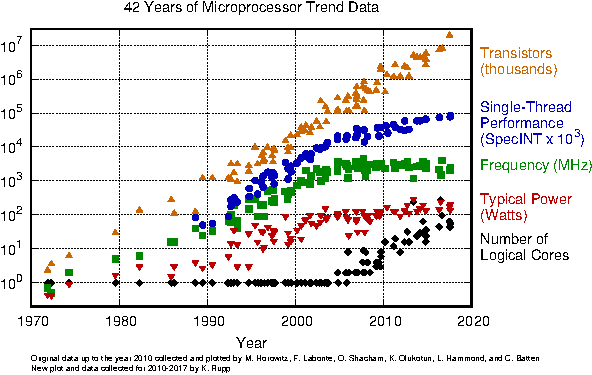
\includegraphics[width=.85\textwidth]{42-years-processor-trend.pdf}%
		\fonte{Adapted from \citeonline{url:microprocessor-trend-data}.}%
	\end{figure}

	% From multicore to manycores and Manycores characteristics
	Yet another classification for manycores is based on
	their ratio between processing speed, measured by the number of \flops, and power consumption,
	in \watts. \autoref{fig:microprocessor-data} pictures that even as the
	number of cores increasing, typical power has not grown uncontrollably.
	For instance, to achieve \exascale ($10^{18}$ \flops), the US Department
	of Defense issued a report stipulating the energy efficiency of a
	supercomputer should be around 50 GFLOPS/\watts~\cite{darpa:exascale}. 
	To cope with this energy constraint, a new class of
	parallel processors, called \textit{\lightweight \manycores}, emerged to
	provide high parallelism with low power consumption.
	Lightweight manycores differ from traditional large-scale
	multicores and manycores in several points: 

	\begin{itemize}
		\item They integrate thousands of low-power cores in a single die organized in clusters;
		\item They are designed to cope with \mimd workloads;
		\item They rely on a high-bandwidth \noc for fast and reliable message-passing communication;
		\item They have constrained memory systems; and
		\item They frequently feature a heterogeneous configuration.
	\end{itemize}

	Some industry-successful examples of \lightweight \manycores are the
	\mppa~\cite{DeDinechin2013-1}; the \epiphany~\cite{olofsson2014};
	and the \taihulight~\cite{zheng2015}. Together with superior performance
	scalability and energy efficiency, lightweight manycores brought a new
	set of challenges in software development coming from their
	architectural particularities. More precisely, these 
	introduced the following difficulties:

	\begin{itemize}
		\item \textit{Hybrid programming model:} due to the parallel and
		distributed nature of the architecture, engineers are frequently
		required to adopt a message-passing programming model to deal
		with the presence of rich \nocs~\cite{kelly2013} that
		interconnects clusters and a shared-memory model inside the
		cluster;

		\item \textit{Missing hardware support for cache coherency:} to
		reduce power consumption, theses processors do not feature cache
		coherency, which in turn forces programmers to handle it
		explicitly in software level and frequently calls out for a
		redesign in their applications~\cite{francesquini2015};

		\item \textit{Constrained memory system:} the frequent presence
		of multiple physical address spaces and small local memories
		require data tiling and prefetching to be handled by the
		software~\cite{Castro2016};

		\item \textit{Heterogeneous configuration:} the different
		programmable components on \lightweight \manycores turns the
		actual deployment of applications in a complex
		task~\cite{barbalace2015}.
	\end{itemize}

	% Challenges and Problem Definition
	Part of these challenges derives from existing runtimes and \oss.
	On the one hand, runtimes do not hide the characteristics of hardware
	making software development more challenging and non-portable, \eg they
	neither allow direct access to non-local data, nor the manipulation of
	them in a transparent way. Thus, fundamental \os mechanisms, such
	as core multiplexing, core partitioning, and process and data
	migration, may not be addressed. On the other hand, the complicated
	portability and scalability of traditional \oss with monolithic
	kernels, which were designed to homogeneous hardware, is leading to
	alternative \os designs~\cite{Baumann2009, kluge2014, nightingale2009, rhoden2011}.

	% Goals and Contributions
	We believe that \oss for the next-generation of \lightweight
	\manycores must be redesigned from scratch to cope with their tight
	architectural constraints. Based on this idea, a new fully-featured
	distributed \os based on a multikernel approach~\cite{Baumann2009}
	is under investigations~\cite{penna2017-1,penna2017-2,penna2019}.
	The \textit{\nanvixmultikernel} features a generic and flexible \hal for
	\lightweight \manycores that addresses the key issues encountered in
	the development for these processors. On top of the \textit{\nanvixhal},
	a microkernel is being designed and implemented to provide the bare bones
	of the most important system abstractions.

\section{Goals}
\label{sec.goals}

	Based on the aforementioned motivations, the primary and specific
	goals of this work are detailed next.

\subsection{Main Goal}
\label{sec.goals.main}

	The main goal of this undergraduate dissertation is to propose an
	\textit{Inter-Cluster Communication Module} to the \textit{\nanvixhal}
	and port it to the \mppa manycore processor~\cite{DeDinechin2013-1}.
	This module exposes the essential abstractions that allow overlying
	layers to create richer communication services. Using this module, we
	also propose \textit{Inter-Cluster Communication Services} to the
	\textit{\nanvixmicrokernel}. This work is part of the collaborative
	project between \ufsc, \pucminas, and \uga to develop an \os for
	\lightweight \manycore platforms.

\subsection{Specific Goals}
\label{sec.goals.specific}

	\begin{itemize}
		\item Definition and proposal of an \textit{Inter-Cluster Communication Interface} for lightweight manycores;

		\item Implementation of the proposed interface in the \textit{\nanvixhal} for the \mppa lightweight manycore processor;
        
		\item Integration of the \nanvixhal interface with the \textit{\nanvixmicrokernel};
		
		\item Performance evaluation of \nanvixmicrokernel implementation using synthetic micro-benchmarks that reproduce the \textit{collective communication routines} of the \mpi programming model.
	\end{itemize}

\section{Organization Of The Work}
\label{sec.organization}

	The remainder of this work is organized as follows.
	In \autoref{ch.background}, we present a background on \os and communication
	design for multicores and multicomputers, the MPPA-256 lightweight manycore
	processor and the Nanvix project.
	In \autoref{ch.related-work}, we discuss the principal related work.
	In \autoref{ch.development}, we discuss the design and implementation
	of the inter-cluster communication facility.
	In \autoref{ch.experiments}, we detail the evaluation methodology
	that we adopted and analyze our experimental results.
	Finally, in \autoref{ch.conclusions}, we draw our conclusions and future work.

\section{Background}

	\subsection{Operating Systems Models}

		\begin{frame}{Models of Operating Systems (OS) for Multicores}
		\begin{overprint}
			\only<1>{
				\begin{itemize}
					\item \textbf{Replicated OS}
					\item Master-Slave OS
					\item Symmetric OS
				\end{itemize}
				\addfig[][width=0.75\linewidth]{replicated-os.pdf}

				\begin{center}
					Each core has a copy of the OS
					Less concurrency but needs a lot of memory
				\end{center}
			}
			\only<2>{
				\begin{itemize}
					\item Replicated OS
					\item \textbf{Master-Slave OS}
					\item Symmetric OS
				\end{itemize}
				\addfig[][width=0.75\linewidth]{master-slave-os.pdf}

				\begin{center}
					Asymmetric execution where only one core handles the OS
					Better scalability but inserts a possible bottleneck
				\end{center}
			}
			\only<3>{
				\begin{itemize}
					\item Replicated OS
					\item Master-Slave OS
					\item \textbf{Symmetric OS}
				\end{itemize}
				\addfig[][width=0.75\linewidth]{symmetric-os.pdf}

				\begin{center}
					OS shared by all cores
					Efficient on cache coherent processors but less scalable
				\end{center}
			}
		\end{overprint}

			% Existem 3 modelos de sistema operacionais para multicores.
			% O primeiro, e mais simples, é o modelo replicado, onde cada núcleo possuem uma cópia distinta do SO. Isso elimina problemas de concorrência mas necessitando de muito espaço de memória.
			% Segundo, o modelo mestre-escravo define que apenas um único núcleo mestre lide com as estruturas do SO, e os escravos requisitem operações a ele. Também eliminando problemas de concorrência mas introduzindo um possível gargalo no sistema.
			% Terceiro, o modelo simétrico é o mais conhecido, ele permite o compartilhamento das estruturas internas forçando o uso de sincronização entre os núcleos do sistema. O que pode ser um problema para processadores que não possuem coerência de cache.
		\end{frame}

	\subsection{Message-Passsing Model}

		% \pholder[Software que lida com interfaces e dma?]{Low-Level Communication}
		\begin{frame}[fragile]{Low-Level Communication for\\Message-Passsing Model}
			\begin{itemize}
				\item \textbf{Computer network concepts}
			\end{itemize}

			\begin{itemize}
				\item Network interfaces
			\end{itemize}

			\begin{itemize}
				\item Performance impacts
				\begin{itemize}
					\item Number of intermediare copies
					\item Direct Memory Access (DMA)
				\end{itemize}
			\end{itemize}

			% Como Lightweight Manycores utilizam uma rede-em-chip para comunicação entre clusters,
			% a comunicação de baixo nível se assemelha a comunicação de uma rede de computadores.
			% Os nós da rede são conectados através de interfaces de rede.
			% O qual tem grande impacto na performace do sistema.
			% Por exemplo, a quantidade de cópias intermediárias ou no uso inadequado de DMAs podem afetar negativamente o desempenho.
		\end{frame}

		% \pholder[Tipos de envio/recebimento?]{User-Level Communication}
		\begin{frame}[fragile]{User-Level Communication for\\Message-Passsing Model}
		\begin{overprint}
			\only<1>{
				\begin{itemize}
					\item Send/receive primitives
					\begin{itemize}
						\item \textbf{Synchronous calls}
						\item Asynchronous calls
					\end{itemize}
				\end{itemize}
				\addfig[][width=.9\linewidth]{call-sync.pdf}
			}
			\only<2>{
				\begin{itemize}
					\item Send/receive primitives
					\begin{itemize}
						\item Synchronous calls
						\item \textbf{Asynchronous calls}
					\end{itemize}
				\end{itemize}
				\addfig[][width=.9\linewidth]{call-async.pdf}
			}
		\end{overprint}

			% Utilizando os recursos de baixo nível, geralmente se exportam primitivas de envio ou recebimento de dados.
			% Essas primitivas podem implementar dois tipos de chamadas.
			% Chamadas síncronas força o requisitante a ficar bloqueado até que toda a operações for concluida.
			% Por outro lado, as chamadas assíncronas permitem que o requisitante continue sua executação após a configuração da primitiva. Isso permite que a síncronzação ocorra a posteriori.
		\end{frame}

	\subsection{Kalray MPPA-256}

		% \pholder[Descrever MPPA]{MPPA-256}
		\begin{frame}[fragile]{Kalray MPPA-256}
			\begin{itemize}
				\item \textbf{High-Performance and Low-Power Consunption}
				\item 288 processing cores
				\begin{itemize}
					\item {16 Compute Cluster (CC)}
					\item {4 I/O Cluster (IO)}
				\end{itemize}
			\end{itemize}
			\addfig[][width=.5\linewidth]{arch-mppa.pdf}

			% O processador MPPA-256 é um Lightweight Manycore de alto desempenho e baixo consumo energético.
			% Ele possui 288 núcleos de propósito geral agrupados em 16 clusters de computação e 4 clusters de entrada e saída.
		\end{frame}

		\begin{frame}[fragile]{Kalray MPPA-256 Communication Resources}
			\begin{itemize}
				\item \textbf{Data NoC (DNoC)}
				\begin{itemize}
					\item 256 slots for receiving data
					\item 8 channels for sending data
					\item 8 $\mu$threads for sending asynchronous data
				\end{itemize}
			\end{itemize}

			\begin{itemize}
				\item \textbf{Control NoC (CNoC)}
				\begin{itemize}
					\item 128 slots for receiving commands
					\item 4 channels for sending commands
				\end{itemize}
			\end{itemize}

			% A comunicação é realizada através de duas NoCs distintas, uma para dados e outra para comandos.
			% Cada NoC apresenta um conjunto de recursos para envio ou recebimento.
			% Entretanto, a CNoC permite apenas a troca de mensagens de 64 bits.
		\end{frame}

	\subsection{Nanvix OS}

		% \pholder{Nanvix OS}
		\begin{frame}[fragile]{Nanvix OS}
			\addfig[][width=.55\linewidth]{nanvix-goal.pdf}

			\begin{itemize}
				\item Fully-feature \textbf{POSIX-Compliant OS}
			\end{itemize}

			\begin{itemize}
				\item \textbf{Three abstractions layers}
				\begin{itemize}
					\item Nanvix Hardware Abstraction Layer (HAL)
					\item Nanvix Microkernel
					\item Nanvix Multikernel
				\end{itemize}
			\end{itemize}

			% O Nanvix OS busca fornecer melhor programabilidade e portabilidade para Lightweight Manycores através de um sistema compatível com o padrão POSIX.
			% Ele é subdivido em três níveis abstração, HAL, Microkernel e Multikernel.
		\end{frame}

		% \pholder{Nanvix HAL}
		\begin{frame}[fragile]{Nanvix HAL}

			\begin{itemize}
				\item \textbf{Generic and flexible} hardware abstraction layer
				\item \textbf{Standard view} of these emerging processors
				\item Proposed interface within \textbf{Processador AL}
			\end{itemize}

			\addfig[][width=.6\linewidth]{nanvix-hal-overview.pdf}

			% A HAL é uma camada de abstração de hardware genérica e flexível.
			% Ela prove uma visão padronizada dos processadores.
			% Ela é composta por níveis que lidam com características de um único núcleo, entre os núcleos, e entre clusters.
			% Este trabalho está incluso na Camada de abstração do Processador, que envolve a interface de comunicação.
		\end{frame}

		% \pholder{Nanvix Microkernel}
		\begin{frame}[fragile]{Nanvix Microkernel}

			\begin{itemize}
				\item Runs above the Nanvix HAL
				\item Provides \textbf{bare-bones of system abstractions}
				\item Follows a \textbf{Master-Slave OS} model
				\item Rich system call interface (Kernel Call)
			\end{itemize}

			\addfig[][width=.6\linewidth]{nanvix-microkernel-overview.pdf}

			% O Nanvix Microkernel executa sobre a HAL e prove o esqueleto das abstrações do sistema.
			% Ele implementa o modelo Mestre-Escravo através de uma rica interface de chamadas de sistema.
			% Desta forma, ele é responsável por gerenciar os recursos da HAL e separar as reponsabilidades de mestre e escravo.
		\end{frame}

		% \pholder{Nanvix Multikernel}
		\begin{frame}[fragile]{Nanvix Multikernel}

			\begin{itemize}
				\item Follows a \textbf{multikernel design}
				\item \textbf{OS services are system processes} and run in isolation
				\item User processes \textbf{request services via message-passing}
			\end{itemize}

			\addfig[][width=.6\linewidth]{nanvix-multikernel-overview.pdf}

			% O Nanvix Multikernel, como o nome sugere, segue o modelo multikernel.
			% No qual os serviços do SO são processos que rodam isoladamente dos processos de usuário.
			% Assim, os processos de usuário requisitam serviços através da troca de mensagens.
		\end{frame}

% LocalWords:  template cls standalone GitHub Overleaf bugfixes SVGs
% LocalWords:  Re-empacotamento fontsize Makefile pdflatex imgs PDFs
% LocalWords:  shell-escape frames SVG brazil english lapesd-slides
% LocalWords:  disabletodonotes todonotes TODO's backup showbackup
% LocalWords:  hidebackup abntexcite abntex natbib nobib titleframe
% LocalWords:  frame showsections sidebar stopcountingframes default
% LocalWords:  thanksframe Thank You Questions referencesframe titulo
% LocalWords:  bibfiles pholder todonote placeholder inline addfig
% LocalWords:  opts graphicx addfiglw width Citations dijkstra Direct
% LocalWords:  Closure Parallel dynamic scheduling DoImportantStuff
% LocalWords:  lccp merged cell svg pdf

\section{Development}

	\subsection{Low-Level Communication}

		\begin{frame}[fragile]{Inter-Cluster Communication Interface}

			\begin{itemize}
				\item Three communication abstractions:
				\begin{itemize}
					\item \textit{Sync}
					\item \textit{Mailbox}
					\item \textit{Portal}
				\end{itemize}
				\item More precise
				\item Easy-to-use
				\item Scalable
				\item Easily portable
			\end{itemize}

			% \textit{\nanvixhal} provides the inter-cluster communication module to allow separate
			% clusters to exchange information.
			% This module consists of three abstractions, named \sync, \mailbox, and \portal.
			% These abstractions provide more precise, easy-to-use, scalable, and easily
			% portable mechanisms for different architectures~\cite{wentzlaff_fleets:_2011}.
			% On top of them, it is possible to create simple facilities, such
			% as those for synchronization and data exchange, as well as more elaborate services
			% like \shm, \posix Semaphores, and \rmem~\cite{penna:rmen}.
		\end{frame}

		% \pholder[Interrup System and DMA mediator]{MPPA-256 Hardware Resources}
		\begin{frame}[fragile]{MPPA-256 Hardware Features}
			\begin{itemize}
				\item Low-level communication depends on two hardware features
				\begin{itemize}
					\item Interrupt System
					\item DMA mediation
				\end{itemize}
				\item Three interrupt lines available
				\item Explicit handler the NoC signals % to identify the resource
				\item DMA limitations
			\end{itemize}
		\end{frame}

		% \pholder{Noc Identifiers}
		\begin{frame}[fragile]{Noc Identifiers}
			\begin{itemize}
				\item NoC interfaces have two identifiers
				\begin{itemize}
					\item Physical ID
					\item Logical ID
				\end{itemize}
			\end{itemize}

			\begin{table}
				\centering%
				\begin{tabular}{l|l|l|}
					\cline{2-3}
											            & \textbf{Physical ID} & \textbf{Logical ID} \\ \hline
					\multicolumn{1}{|l|}{\textbf{IO 0}} & 128-131              & 0-3                 \\ \hline
					\multicolumn{1}{|l|}{\textbf{IO 1}} & 192-195              & 4-7                 \\ \hline
					\multicolumn{1}{|l|}{\textbf{CCs}}  & 0-15                 & 8-23                \\ \hline
				\end{tabular}
			\end{table}
		\end{frame}

		% \pholder{Resource Identifiers}
		\begin{frame}[fragile]{Resource Identifiers}
			\begin{itemize}
				\item Senders need to know \textbf{resource ID} of the destination interface
				\item Communication resources are \textbf{partitioned by abstraction}
			\end{itemize}

			\begin{table}[!tb]
				\centering%
				\begin{tabular}{l|l|l|l|l|}
					\cline{2-5}
														   & \multicolumn{2}{c|}{\textbf{CNoC}}               & \multicolumn{2}{c|}{\textbf{DNoC}}           \\ \cline{2-5}
														   & \textbf{RX ID} & \textbf{TX ID} & \textbf{RX ID} & \textbf{TX ID} \\ \hline
					\multicolumn{1}{|l|}{\textbf{Mailbox}} & 0-23           & 0              & 0-23           & 1-3            \\ \hline
					\multicolumn{1}{|l|}{\textbf{Portal}}  & 24-47          & 1-2            & 24-47          & 4-7            \\ \hline
					\multicolumn{1}{|l|}{\textbf{Sync}}    & 48-71          & 3              & -              & -              \\ \hline
				\end{tabular}
			\end{table}
		\end{frame}

		% \pholder[Lazy transfer and Interface convention]{General Concepts of Comm. Abstrations}
		\begin{frame}[fragile]{General Concepts of Comm. Abstrations}
			\begin{itemize}
				\item Master core cannot be blocked
				\item Communication Interfaces export only asynchronous calls
				\item Slaves wait Master core complete a task
				\item \textbf{Lazy transfer algorithm}
				\item Naming Convention
				\begin{itemize}
					\item Sender Role: \texttt{create}/\texttt{unlink}/\texttt{aread}/\texttt{wait}
					\item Receiver Role: \texttt{open}/\texttt{close}/\texttt{awrite/signal}/\texttt{wait}.
				\end{itemize}
			\end{itemize}
			% The microkernel specifically assigns the master core the task
			% of handling requests (\ie kernel calls) from slave cores. Therefore,
			% interfaces export only asynchronous calls. This decision forces
			% the upper layer, if desired, to create synchronous calls that
			% call the wait function right after the asynchronous operation.
			% Thus, at the microkernel level, we can ensure that the master core
			% sets or executes asynchronous functions and notifies blocked slaves.

			% \autoref{alg:lazy-transfer} illustrates the behavior of
			% lazy transfer, the algorithm defines that the master saves the
			% parameters of transmission if it does not have desired permission
			% and will accomplish other requests. Upon receiving permission
			% from the receiver, the interrupt handler identifies the resource,
			% actually sends the data and releases the slave that requested the
			% send. This algorithm ensures that the master is always doing useful
			% operations and never crashes the entire system.

			% Finally, abstract interfaces follow a convention to distinguish
			% between receiver and sender roles. Receivers use functions with
			% \texttt{create}, \texttt{unlink}, \texttt{aread}, and \texttt{wait}
			% suffixes. Senders, in turn, use functions with \texttt{open},
			% \texttt{close}, \texttt{awrite/signal}, and \texttt{wait} suffixes.
			% Because the \texttt{wait} function is shared, the abstraction must
			% distinguish the role by the resource identifier. Discriminating the
			% nature of operations helps both the user, being entirely intuitive,
			% and implementing \hal by explaining what features will be needed.
		\end{frame}

		% \pholder[Concept]{Sync Abstration Concept}
		\begin{frame}[fragile]{Sync Abstration}
			\begin{overprint}
			\only<1>{
				\begin{itemize}
					\item Provides cluster synchronization across \textbf{distributed barriers}
					\item Analogous to POSIX Signals
					\item Two modes
					\begin{itemize}
						\item \textbf{\texttt{ALL\_TO\_ONE}}
						\item \texttt{ONE\_TO\_ALL}
					\end{itemize}
				\end{itemize}
				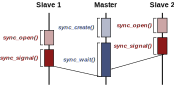
\includegraphics[width=.75\linewidth]{imgs/sync-all-to-one.pdf}
			}
			\only<2>{
				\begin{itemize}
					\item Provides cluster synchronization across \textbf{distributed barriers}
					\item Analogous to POSIX Signals
					\item Two modes
					\begin{itemize}
						\item \texttt{ALL\_TO\_ONE}
						\item \textbf{\texttt{ONE\_TO\_ALL}}
					\end{itemize}
				\end{itemize}
				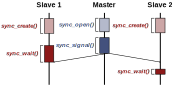
\includegraphics[width=.75\linewidth]{imgs/sync-one-to-all.pdf}
			}
		\end{overprint}

			% \textit{Synchronization Abstraction}, called \sync, provides the
			% basis for cluster synchronization across distributed barriers.
			% Its behavior is analogous to \posix Signals abstraction, but
			% notifications do not carry information, they are only for synchronization.
			% \sync defines two synchronization modes, \texttt{ALL\_TO\_ONE} and
			% \texttt{ONE\_TO\_ALL}. In both modes, there is a single master node
			% (\texttt{ONE}) and one or more slave nodes
			% (\texttt{ALL}) involved in the communication. \autoref{fig:sync-all-to-one} illustrates the
			% \texttt{ALL\_TO\_ONE} mode, where the master node waits blocked for
			% the $N$ notifications coming from the slaves. In contrast,
			% \autoref{fig:sync-one-to-all} pictures the \texttt{ONE\_TO\_ALL} mode,
			% where the master notifies the $N$ slaves, releasing them from the lock.
			% The sender nodes are responsible for sending a signal and will never
			% block. Receiver nodes are responsible for waiting for all notifications
			% to arrive.
		\end{frame}

		% \pholder[Implementation]{Sync Abstration Implementation}
		\begin{frame}[fragile]{Sync Abstration Implementation}
			\begin{itemize}
				\item Parameters required
				\begin{itemize}
					\item Node list
					\item List size
					\item Mode
				\end{itemize}
				\item Master node must be the first on the list
			\end{itemize}

			\begin{itemize}
				\item Resources required
				\begin{itemize}
					\item Create: 1 RX CNoC
					\item Open: 1 TX CNoC
				\end{itemize}
			\end{itemize}

			\begin{itemize}
				\item Simultaneous operations
				\begin{itemize}
					\item Create: 24
					\item Open: 1
				\end{itemize}
			\end{itemize}
		\end{frame}

		% \pholder[Concept]{Mailbox Abstration Concept}
		\begin{frame}[fragile]{Mailbox Abstration}
			\begin{itemize}
				\item Allows exchange fixed-length message
				\item Similarly to POSIX Message Queue
				\item Receiver allocates space to N messages
				\item Sender transfer to predefined location
			\end{itemize}

			\addfig[][width=.5\linewidth]{mailbox-concept.pdf}
			\addfig[][width=.5\linewidth]{mailbox-flow.pdf}			

			% \textit{Message Queue Abstraction}, called \mailbox, allows clusters to exchange
			% fixed-length messages with each other. The message size is designed to be
			% relatively small, usually a few hundreds of bytes. The recipient consumes these
			% messages without needing to know who sent them. Similarly, mailbox operations
			% follow the behavior of the \posix message queue. \autoref{fig:mailbox-concept}
			% conceptually illustrates one of the ways to implement a \mailbox. The receiver
			% allocates enough space to receive one message from each possible sender.
			% The sender transfers the message to a predefined location.

			% \autoref{fig:mailbox-flow} outlines the communication flow between a
			% receiver and a sender node. The receiver creates an empty message queue
			% where senders are free to send the first message. Subsequently, to
			% avoid overwriting old messages, all transmissions require the permission
			% of the receiver. For this reason,  when the receiver consumes a message,
			% it copies the message to the user buffer, releases the queue space, and
			% notifies the sender.
		\end{frame}

		% \pholder[Implementation]{Mailbox Abstration Implementation}
		\begin{frame}[fragile]{Mailbox Abstration Implementation}
			\begin{itemize}
				\item Parameters required
				\begin{itemize}
					\item Node list
					\item List size
					\item Mode
				\end{itemize}
				\item Master node must be the first on the list
			\end{itemize}

			\begin{itemize}
				\item Resources required
				\begin{itemize}
					\item Create: 1 RX CNoC
					\item Open: 1 TX CNoC
				\end{itemize}
			\end{itemize}

			\begin{itemize}
				\item Simultaneous operations
				\begin{itemize}
					\item Create: 24
					\item Open: 1
				\end{itemize}
			\end{itemize}
		\end{frame}

		\pholder[Concept]{Portal Abstration Concept}

		% \pholder[Implementation]{Portal Abstration Implementation}
		\begin{frame}[fragile]{Portal Abstration Implementation}
			\begin{itemize}
				\item Parameters required
				\begin{itemize}
					\item Node list
					\item List size
					\item Mode
				\end{itemize}
				\item Master node must be the first on the list
			\end{itemize}

			\begin{itemize}
				\item Resources required
				\begin{itemize}
					\item Create: 1 RX CNoC
					\item Open: 1 TX CNoC
				\end{itemize}
			\end{itemize}

			\begin{itemize}
				\item Simultaneous operations
				\begin{itemize}
					\item Create: 24
					\item Open: 1
				\end{itemize}
			\end{itemize}
		\end{frame}

	\subsection{User-Level Communication}

		\pholder{Impacts of the Master-Slave Model}

		\pholder[Protection and Management, Multiplexing, Validation and Correctness Tests]{Details}

% LocalWords:  template cls standalone GitHub Overleaf bugfixes SVGs
% LocalWords:  Re-empacotamento fontsize Makefile pdflatex imgs PDFs
% LocalWords:  shell-escape frames SVG brazil english lapesd-slides
% LocalWords:  disabletodonotes todonotes TODO's backup showbackup
% LocalWords:  hidebackup abntexcite abntex natbib nobib titleframe
% LocalWords:  frame showsections sidebar stopcountingframes default
% LocalWords:  thanksframe Thank You Questions referencesframe titulo
% LocalWords:  bibfiles pholder todonote placeholder inline addfig
% LocalWords:  opts graphicx addfiglw width Citations dijkstra Direct
% LocalWords:  Closure Parallel dynamic scheduling DoImportantStuff
% LocalWords:  lccp merged cell svg pdf

\section{Experiments}

	% \pholder{Methodology}
	\begin{frame}[fragile]{Methodology}
		\begin{itemize}
			\item Evaluation of the performance of \textbf{data transfer services}
			\begin{itemize}
				\item Mailbox
				\item Portal
			\end{itemize}
			\item Micro-benchmarks stimulate the services with well-known \textbf{collective communication routines}
		\end{itemize}

		% Os experimentos realizados buscaram avaliar os serviços de transferência de dados, como mailbox e portal.
		% Entretanto, o sync foi utilizado para realizar a sincronização de todos os clusters envolvidos.
		% Para prover uma avaliação abrangente, os micro-benchmarks estimularam os serviços usando rotinas de comunicação coletivas.
	\end{frame}

	% \pholder{Micro-benchmarks}
	\begin{frame}[fragile]{Micro-benchmarks}
		\begin{overprint}
			\only<1>{
				\begin{itemize}
					\item \textbf{Broadcast}
					\item Gather
					\item AllGather
					\item Ping-Pong
				\end{itemize}
				\addfig[][width=.5\linewidth]{mpi-broadcast.pdf}
			}
			\only<2>{
				\begin{itemize}
					\item Broadcast
					\item \textbf{Gather}
					\item AllGather
					\item Ping-Pong
				\end{itemize}
				\addfig[][width=.5\linewidth]{mpi-gather.pdf}
			}
			\only<3>{
				\begin{itemize}
					\item Broadcast
					\item Gather
					\item \textbf{AllGather}
					\item Ping-Pong
				\end{itemize}
				\addfig[][width=.5\linewidth]{mpi-allgather.pdf}
			}
			\only<4>{
				\begin{itemize}
					\item Broadcast
					\item Gather
					\item AllGather
					\item \textbf{Ping-Pong}
				\end{itemize}
				\addfig[][width=.5\linewidth]{mpi-ping-pong.pdf}
			}
		\end{overprint}

		% Ao todo foram implementados 4 rotinas.
		% A rotina broadcast define um nó mestre enviando uma mesma mensagem para N escravos.
		% Opostamente, a rotina gather, define que todos os escravos enviem seus dados para o mestre.
		% A rotina AllGather é uma generalização do gather, no qual todos enviam e recebem dados de todos mundo.
		% Por fim, a rotina Ping-Pong representa as diversas requisições e respostas de um modelo cliente-servidor.
	\end{frame}

	% \pholder{Design}
	\begin{frame}[fragile]{Experimental Design}
		\begin{itemize}
			\item \textbf{Throughput of the Portal}
			\begin{itemize}
				\item Constant: 1 IO and 16 CCs
				\item Variable: 4, 8, 16, 32, 64 KB
			\end{itemize}
			\item \textbf{Latency of the Mailbox}
			\begin{itemize}
				\item Variable: 1 IO and 1 to 16 CCs
				\item Constant: 120 B
			\end{itemize}
			\item \textbf{50 iterations}, discarding first ten
			\item Standard error inferior to \textbf{1\%}
		\end{itemize}

		% Para o serviço do Portal, foi avaliado a taxa de transferência de dados envolvendo sempre um número fixo de cluster. O que variou a quantidade de dados, variando de 4 KB até 64 KB.
		% Já a latência da mailbox envolveu um número variável de clusters porque a mensagem trocada é fixada com o tamanho de 120 bytes.
		% Todos os experimentos tiveram 50 iterações, mas as 10 primeiras foram descartadas para ignorar variações provenientes da inicialização do experimento.
		% Por fim, todos os resultados obtiveram erro padrão menor que 1%.
	\end{frame}

	% \pholder{Portal Analysis}
	\begin{frame}[fragile]{Portal Analysis}
		\addfig[][width=.9\linewidth]{portal-throughput.pdf}

		% O gráfico mostra a taxa de transferência do Portal em MB/s relativo a quantidade de dados transferido.
		% Os resultados exibiram três comportamentos distintos.
		% O primeiro, o broadcast apresentou os piores resultados como experado, por causa do único emissor envolvido.
		% Segundo, Gather e Ping-Pong estão sobrepostos porque tiveram resultados similares.
		% Isso é causado por causa da serialização das leituras pelo mestre, o qual dita o fluxo dos dados.
		% Terceiro, o melhor dos resultados foi do AllGather, porque as comunicações ocorriam em pares de nós, o que permite o paralelismo das tranferências.
		% No contexto de Sistems Operacionais, onde teremos subsistemas requisitando grandes transferências de dados, como um sistema de paginação, podemos inferir que tamanhos entre 8 e 16 KB favorecem a taxa de transferência do Portal.
		% Apesar de tudo, acreditamos que ao eliminar as limitações da DMA, o Portal deve ter ganhos significativos.
	\end{frame}

	% \pholder{Mailbox Analysis}
	\begin{frame}[fragile]{Mailbox Analysis}
		\addfig[][width=.9\linewidth]{mailbox-latency.pdf}

		% Por outro lado, o gráfico da Mailbox apresenta a latencia em milisegundos relativo ao número de clusters de computação envolvidos.
		% Primeiramente, as rotinas Gather e AllGather apresentaram os melhores resultados por causa do  paralelismo do recebimento das N mensagens. A diferença do AllGather se encontra na necessidade de envio e leitura, diferente da Gather.
		% Segundo, o broadcast sofreu do mesmo mal da rotina no Portal, por causa do único emissor de mensagens.
		% Por último, o ping-pong apresentou os piores resultados, onde é possível notar que seus resultados são similares as somas dos resultados do gather e do broadcast.
		% O que indica que o ganho do mestre em receber as mensagens em paralelo foi atenuado pelo gargalo de enviar N mensagens.
		% Entretanto, de forma geral, os resultados mostraram que é possível suportar de forma eficiente essas rotinas no Nanvix Multikernel. Os resultados do Ping-pong, por sua vez, mostraram potenciais melhorias que devem ser estudadas na comunicação dos subsistemas do Nanvix.
	\end{frame}

% LocalWords:  template cls standalone GitHub Overleaf bugfixes SVGs
% LocalWords:  Re-empacotamento fontsize Makefile pdflatex imgs PDFs
% LocalWords:  shell-escape frames SVG brazil english lapesd-slides
% LocalWords:  disabletodonotes todonotes TODO's backup showbackup
% LocalWords:  hidebackup abntexcite abntex natbib nobib titleframe
% LocalWords:  frame showsections sidebar stopcountingframes default
% LocalWords:  thanksframe Thank You Questions referencesframe titulo
% LocalWords:  bibfiles pholder todonote placeholder inline addfig
% LocalWords:  opts graphicx addfiglw width Citations dijkstra Direct
% LocalWords:  Closure Parallel dynamic scheduling DoImportantStuff
% LocalWords:  lccp merged cell svg pdf

\section{Conclusions}

	% \pholder[Quais foram as conclusões?]{Conclusions}
	\begin{frame}[fragile]{Conclusions}
		\begin{itemize}
			\item Historical evolution of processors
			\item Concern about relationship between \textbf{processing power and power consumption}
			\item Arising of \textbf{Lightweight Manycores}
			\item Design of Inter-Cluster Communication Facility
			\begin{itemize}
				\item Sync
				\item Mailbox
				\item Portal
			\end{itemize}
			\item Well-known \textbf{distributed algorithms can be efficiently supported} by Nanvix OS 
		\end{itemize}
		
		% Este trabalho apresentou a evolução dos processadores monocores até os manycores atuais.
		% Expôs a crescente preocupação da relação entre poder de processamento e consumo de energia.
		% O que levou o surgimento dos Lightweight Manycores.
		% O desenvolvimento envolveu o projeto de mecanismos de comunicação e, através de experimentos, mostrou-se como algoritmos distribuídos conhecidos podem ser eficientemente suportados pelo Nanvix OS. 		
	\end{frame}

	% \begin{frame}[fragile]{Future Works}
	% 	\begin{itemize}
	% 		\item Eliminates DMA limitation
	% 		\item Enhancements Ping-Pong performace
	% 		\item Implements MPI
	% 	\end{itemize}
	% \end{frame}

% LocalWords:  template cls standalone GitHub Overleaf bugfixes SVGs
% LocalWords:  Re-empacotamento fontsize Makefile pdflatex imgs PDFs
% LocalWords:  shell-escape frames SVG brazil english lapesd-slides
% LocalWords:  disabletodonotes todonotes TODO's backup showbackup
% LocalWords:  hidebackup abntexcite abntex natbib nobib titleframe
% LocalWords:  frame showsections sidebar stopcountingframes default
% LocalWords:  thanksframe Thank You Questions referencesframe titulo
% LocalWords:  bibfiles pholder todonote placeholder inline addfig
% LocalWords:  opts graphicx addfiglw width Citations dijkstra Direct
% LocalWords:  Closure Parallel dynamic scheduling DoImportantStuff
% LocalWords:  lccp merged cell svg pdf


%%%%%%%%%%%%%%%%%%%%%%%%%%%%
% Finalização
%%%%%%%%%%%%%%%%%%%%%%%%%%%%

\thanksframe
\referencesframe{references}

\begin{backup}
  \pholder{Slide de backup}
\end{backup}

% LocalWords:  template cls standalone GitHub Overleaf bugfixes SVGs
% LocalWords:  Re-empacotamento fontsize Makefile pdflatex imgs PDFs
% LocalWords:  shell-escape frames SVG brazil english lapesd-slides
% LocalWords:  disabletodonotes todonotes TODO's backup showbackup
% LocalWords:  hidebackup abntexcite abntex natbib nobib titleframe
% LocalWords:  frame showsections sidebar stopcountingframes default
% LocalWords:  thanksframe Thank You Questions referencesframe titulo
% LocalWords:  bibfiles pholder todonote placeholder inline addfig
% LocalWords:  opts graphicx addfiglw width Citations dijkstra Direct
% LocalWords:  Closure Parallel dynamic scheduling DoImportantStuff
% LocalWords:  lccp merged cell svg pdf


\end{document}

% LocalWords:  template cls standalone GitHub Overleaf bugfixes SVGs
% LocalWords:  Re-empacotamento fontsize Makefile pdflatex imgs PDFs
% LocalWords:  shell-escape frames SVG brazil english lapesd-slides
% LocalWords:  disabletodonotes todonotes TODO's backup showbackup
% LocalWords:  hidebackup abntexcite abntex natbib nobib titleframe
% LocalWords:  frame showsections sidebar stopcountingframes default
% LocalWords:  thanksframe Thank You Questions referencesframe titulo
% LocalWords:  bibfiles pholder todonote placeholder inline addfig
% LocalWords:  opts graphicx addfiglw width Citations dijkstra Direct
% LocalWords:  Closure Parallel dynamic scheduling DoImportantStuff
% LocalWords:  lccp merged cell svg pdf
